\documentclass[aspectratio=169, handout]{beamer}
%\documentclass[aspectratio=169]{beamer}


\makeatletter
\renewcommand*\env@matrix[1][\arraystretch]{%
  \edef\arraystretch{#1}%
  \hskip -\arraycolsep
  \let\@ifnextchar\new@ifnextchar
  \array{*\c@MaxMatrixCols c}}
\makeatother

\usepackage{tikz}
\usetikzlibrary{tikzmark,fit,shapes.geometric}


\newcommand{\transp}{^{\rm{T}}}

\usepackage{cases}
\usepackage[english]{babel}
% or whatever
\usepackage{xcolor}
\usepackage{colortbl}
\usepackage[latin1]{inputenc}
\usepackage[super]{nth}
% or whatever
%\setbeamertemplate{footline}[page number]
\setbeamertemplate{footline}
        {
      \leavevmode%
      \hbox{%
      \begin{beamercolorbox}[wd=.333333\paperwidth,ht=2.25ex,dp=1ex,center]{author in head/foot}%
        \usebeamerfont{author in head/foot}\insertshortauthor%~~(\insertshortinstitute)
      \end{beamercolorbox}%
      \begin{beamercolorbox}[wd=.333333\paperwidth,ht=2.25ex,dp=1ex,center]{title in head/foot}%
        \usebeamerfont{title in head/foot}\insertshorttitle
      \end{beamercolorbox}%
      \begin{beamercolorbox}[wd=.333333\paperwidth,ht=2.25ex,dp=1ex,right]{date in head/foot}%
        \usebeamerfont{date in head/foot}\insertshortdate{}\hspace*{2em} \insertframenumber{}  \hspace*{2em}%/ \inserttotalframenumber\hspace*{2ex} 

    %#turning the next line into a comment, erases the frame numbers
        

      \end{beamercolorbox}}%
      \vskip 0pt%
    }

\usepackage{times}
\usepackage[T1]{fontenc}
\usepackage{psfrag}
\usepackage{algorithm}
\usepackage{amsmath}
\usepackage{amssymb}
\usepackage{tabularx}
\usepackage{algpseudocode}
\usepackage{mathrsfs}
\usepackage{textpos}
\usepackage{graphicx}
\usepackage{tcolorbox}
\usepackage{multicol}
\usepackage{tikz}
\usetikzlibrary{arrows.meta,shapes.arrows}
%\setkeys{Gin}{draft}
\usepackage{caption}
\captionsetup{font=scriptsize,labelfont=scriptsize}
\usepackage{color}
\DeclareCaptionFont{blue}{\color{blue}}
\captionsetup{labelfont=blue}
\usepackage{tikz}
\tikzset{
  every overlay node/.style={
    draw=white,anchor=north west,
  },
}
\def\checkmark{\tikz\fill[scale=0.4](0,.35) -- (.25,0) -- (1,.7) -- (.25,.15) -- cycle;}
\def\tikzoverlay{%
   \tikz[baseline,overlay]\node[every overlay node]
}%
%\DeclareGraphicsRule{.png}{png}{.png.bb}{}

\newtheorem{assumption}{Assumption} %jw

\newcommand{\T}{{\rm T}}

\newcommand\blfootnote[1]{%
  \begingroup
  \renewcommand\thefootnote{}\footnote{#1}%
  \addtocounter{footnote}{-1}%
  \endgroup
}
\setcounter{tocdepth}{1}
\beamertemplatenavigationsymbolsempty


\title[Lecture 12: Gradient Descent] % (optional, use only with long paper titles)
{Data, Environment and Society: \\{Lecture 12: Gradient Descent}}


%\subtitle
%{Include Only If Paper Has a Subtitle}

\author[ER131: Data, Environment and Society] 
{Instructor: Duncan Callaway\\
GSI: Salma Elmallah} 
% - Give the names in the same order as the appear in the paper.
% - Use the \inst{?} command only if the authors have different
%   affiliation.

%\logo{
%\includegraphics[width=1.5cm,height=1.5cm,keepaspectratio]{uvic_logo_h.jpg}
%}
\vspace{-20mm}
\institute[UC Berkeley] % (optional, but mostly needed)
 {\small{ \bf October 8, 2019}}


\date[October 8, 2019]


\begin{document}

\begin{frame}[plain, noframenumbering]
  \titlepage
\end{frame}

\begin{frame}{Announcements}

\textbf{Today}
\begin{itemize}
\item Gradient descent, a.k.a. how to use computers to do better than the normal equations
\item Discuss Novotny \textit{et al}
\end{itemize}

\textbf{Next time}
\begin{itemize}
\item Resampling, a.k.a. how to use computers to do better than AIC.
\item Bring your laptop!
\end{itemize}

\textbf{Reading}
\begin{itemize}
\item Today: Novotny \textit{et al}; Ch 11 DS100
\item Next time: ISLR 5.1-5.2
\end{itemize}
\end{frame}


\begin{frame}[t]

\begin{columns}

\column{0.25\textwidth}
\begin{figure}
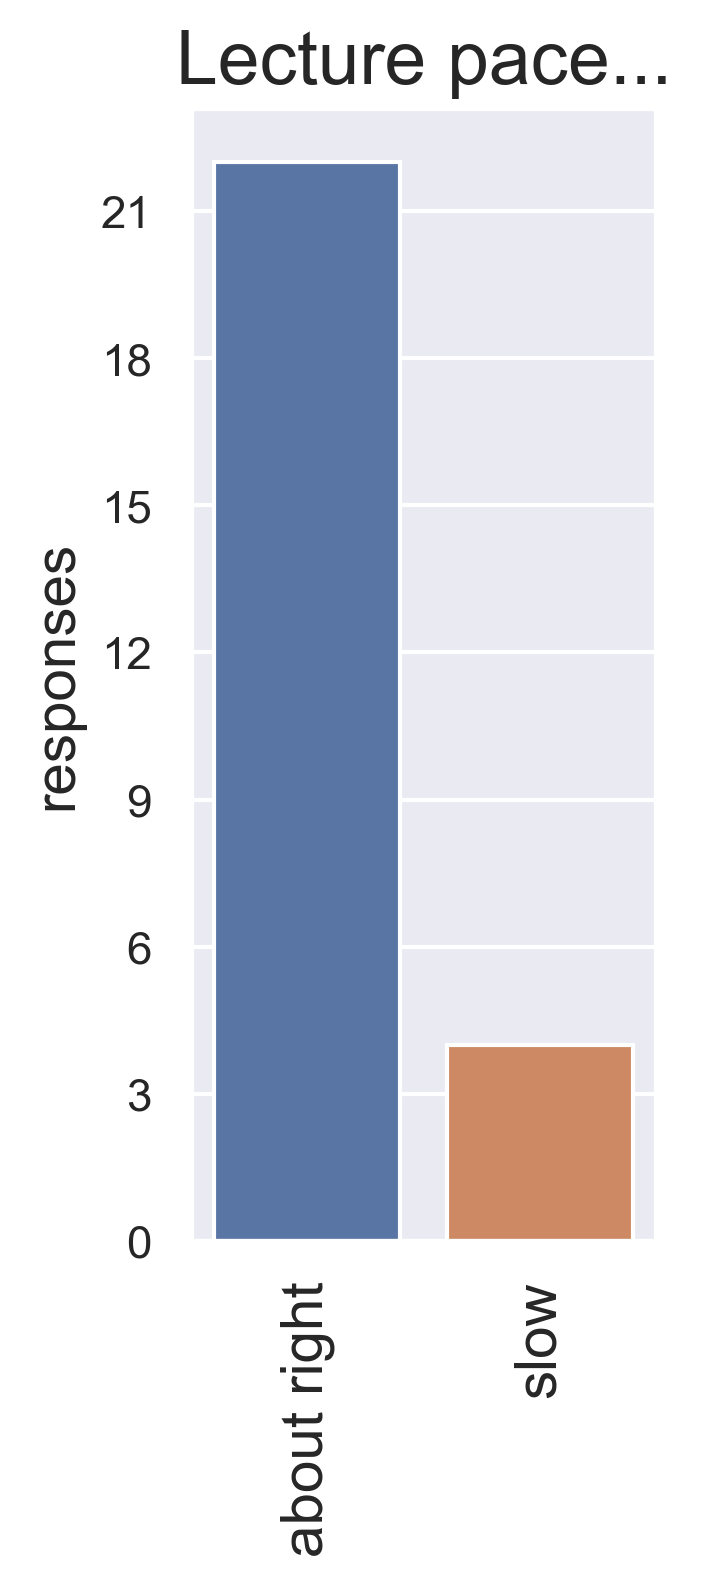
\includegraphics[width=0.9\textwidth]{survey_pace}
\caption*{}
\end{figure}

\column{0.25\textwidth}
\begin{figure}
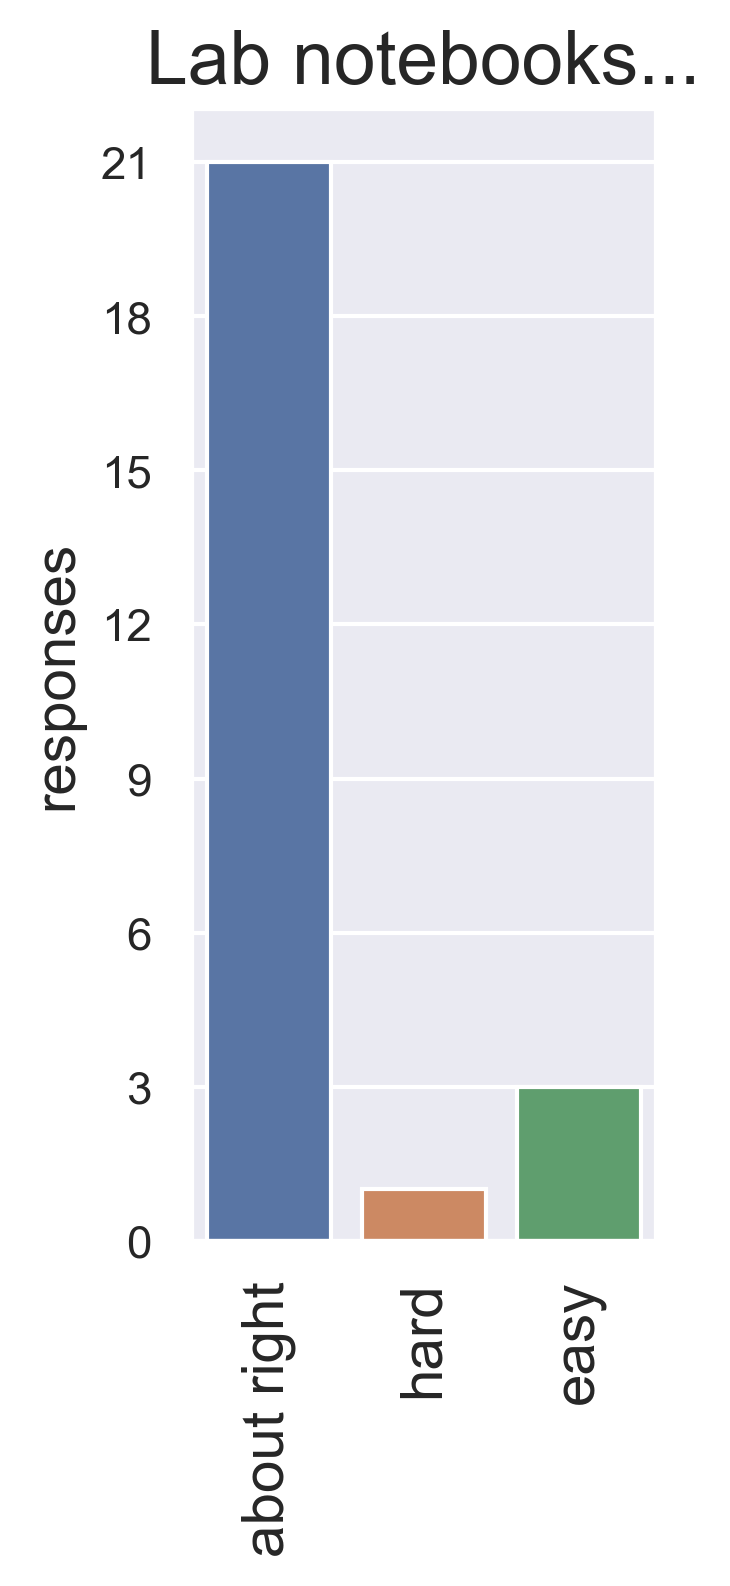
\includegraphics[width=0.9\textwidth]{survey_lab_notebooks}
\caption*{}
\end{figure}

\column{0.25\textwidth}
\begin{figure}
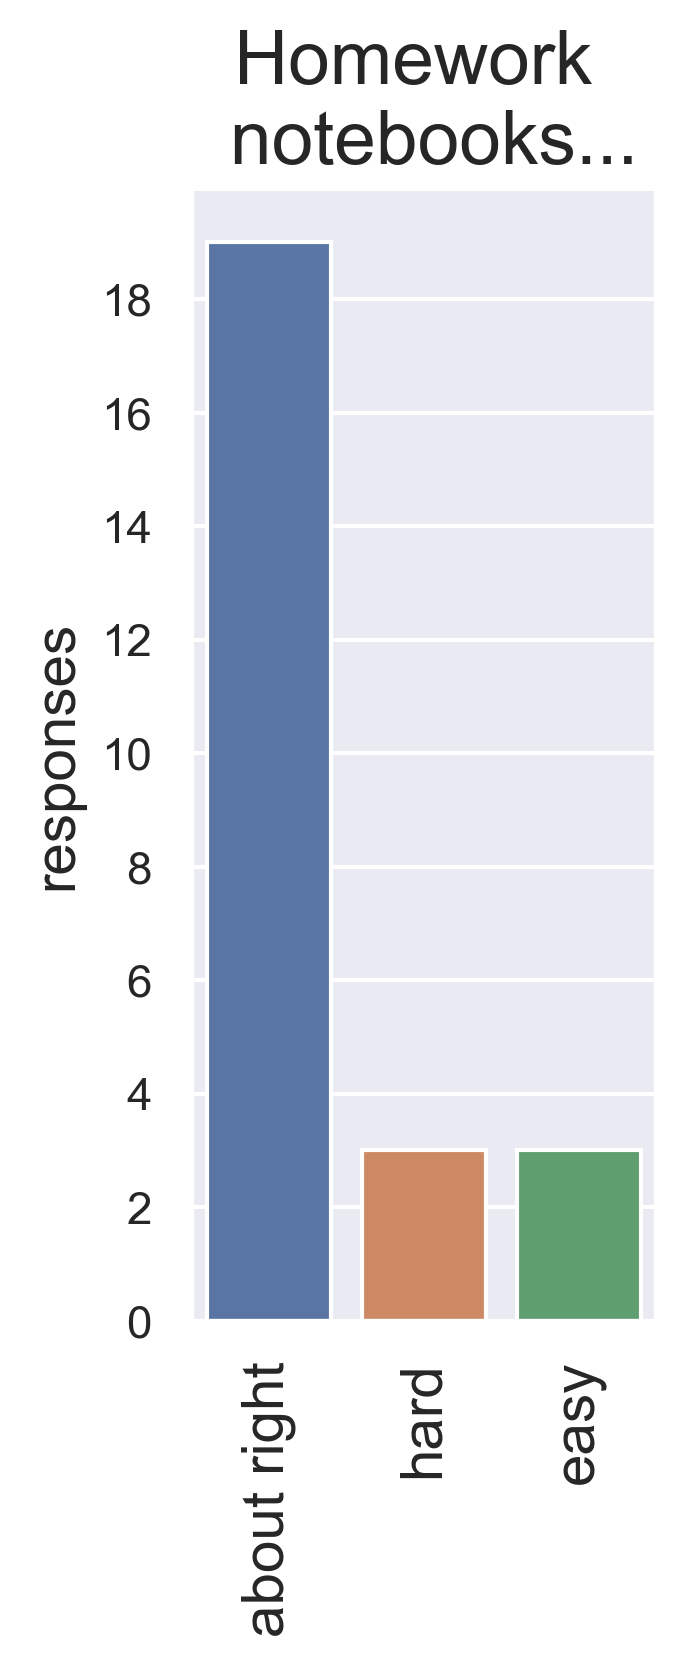
\includegraphics[width=0.9\textwidth]{survey_hw}
\caption*{}
\end{figure}

\column{0.25\textwidth}
\begin{figure}
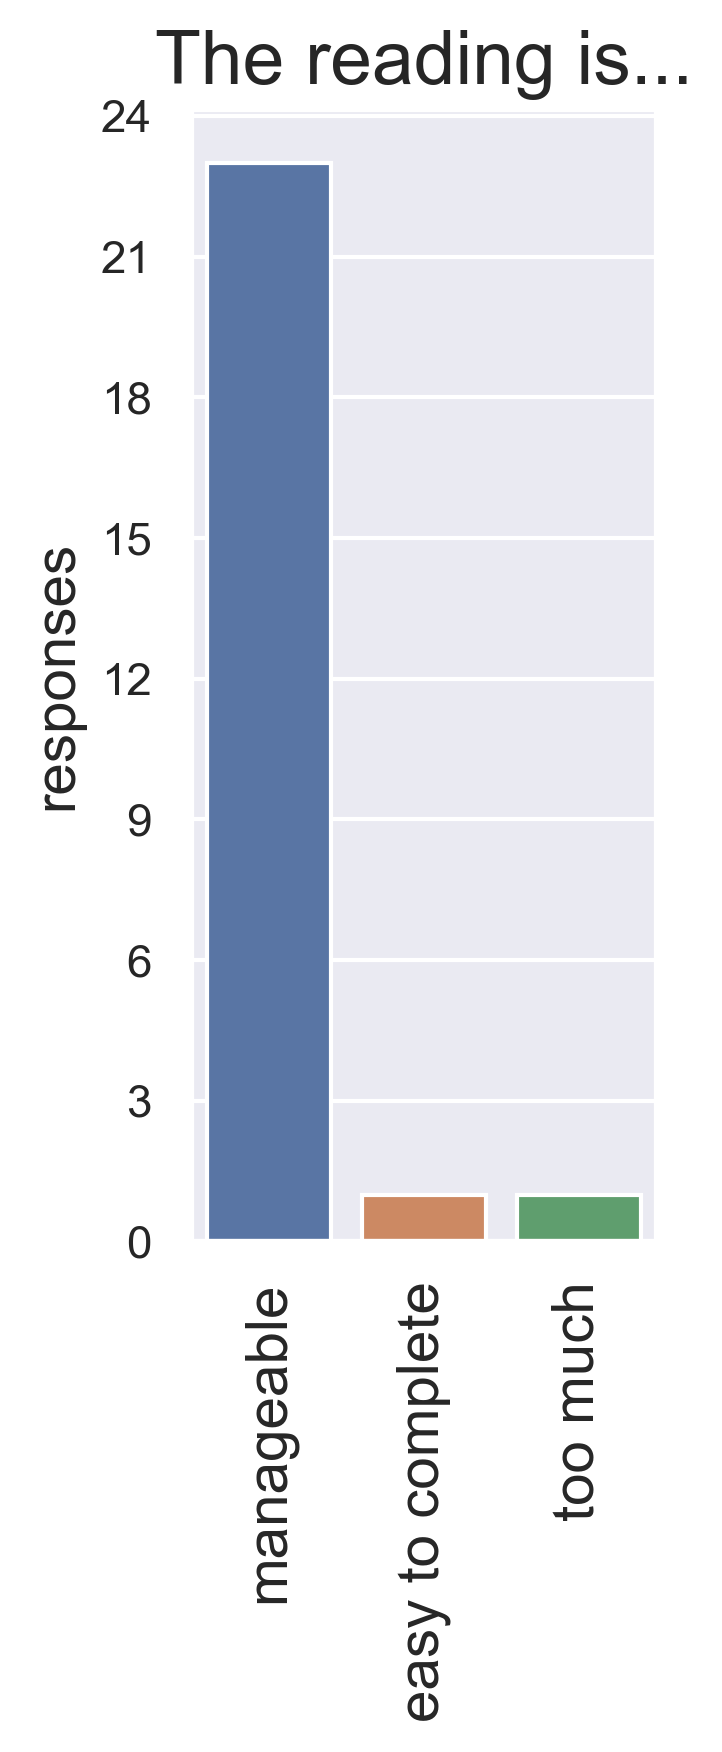
\includegraphics[width=0.9\textwidth]{survey_readings}
\caption*{}
\end{figure}

\end{columns}
\end{frame}


\begin{frame}{Basic estimation process, so far}
\begin{enumerate}
\item Define a ``loss function''
\item Set derivatives of loss function equal to zero and solve for parameters
\end{enumerate}

\vspace{5mm}
The challenge:
\begin{itemize}
\item Setting loss function derivatives to zero not always easy.
\item This doesn't scale well for big problems (e.g. many different nonlinear transformations of the Novotny data)
\end{itemize}
\end{frame}

\begin{frame}{The ``constant'' model}

On the next few slides we're be talking about the so-called constant model.

\vspace{5mm}

Consider a basic linear model.  We're familiar with this one:
\uncover<2->{\begin{align*}
  \hat{y_i} = \theta + \beta x_i
\end{align*}}

The constant model just forces $\beta = 0$:
\uncover<2->{\begin{align*}
  \hat{y_i} = \theta
\end{align*}}

In words: The model is that all observations are actually the same value.  

\vspace{5mm}

Of course in a lot of cases this will be a terrible model, but it has interesting properties, as we'll see.


\end{frame}

\begin{frame}{The loss function}

Mean squared error, aka the `L2' norm
\uncover<2->{
	\begin{align*}
		\text{MSE} &= \frac{1}{n}\sum_{i=1}^n (y_i - \hat{y}_i)^2\\
		\text{Constant model} \rightarrow \text{MSE} &= \frac{1}{n}\sum_{i=1}^n (y_i - {\theta})^2\\
	\end{align*}
}
Mean absolute error, aka the `L1' norm
\uncover<2->{
	\begin{align*}
		\text{MAE} &= \frac{1}{n}\sum_{i=1}^n |y_i - \hat{y}_i|\\
		\text{Constant model} \rightarrow \text{MAE} &= \frac{1}{n}\sum_{i=1}^n |y_i - {\theta}|
	\end{align*}
}

\end{frame}

\begin{frame}{Advantages and disadvantages to MAE and MSE?}
\begin{figure}
	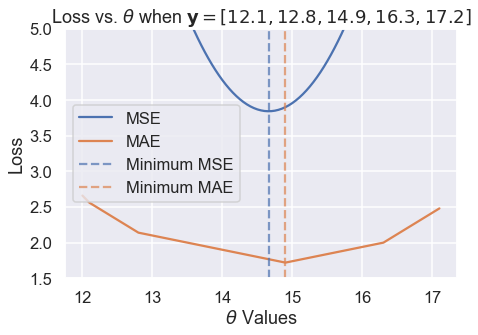
\includegraphics[width=0.5\textwidth]{mae_vs_mse}
	\caption*{}
\end{figure}
\pause
\vspace{-10mm}
\begin{itemize}
	\item MSE is differentiable $\rightarrow$ can solve directly for coefficients
	\item MAE is less impacted by extreme values
\end{itemize}
\end{frame}

\begin{frame}{Aside: what do these cost functions provide with the ``constant'' model?}

What well-known values minimize these loss functions?

	\begin{align*}
		\theta^*_{\text{MSE}} = \arg \min_\theta  \frac{1}{n}\sum_{i=1}^n (y_i - \theta)^2\\
		\theta^*_{\text{MAE}} = \arg \min_\theta  \frac{1}{n}\sum_{i=1}^n |y_i - \theta|
	\end{align*}

\end{frame}

\begin{frame}{Mean absolute error, solution}

\uncover<2->{
  \begin{align*}
    L &= \frac{1}{n}\sum_{i=1}^n (y_i - \theta)^2\\
    \frac{\partial L}{\partial \theta} &= \frac{2}{n} \left(\sum_{i =1}^n  y_i - \theta \right) =\frac{2}{n} \left(\sum_{i =1}^n  y_i\right) - 2\theta   \\
    \frac{\partial L}{\partial \theta} &=0 \rightarrow 2\theta = \frac{2}{n} \left(\sum_{i =1}^n  y_i\right)\\
    \rightarrow \theta &= \frac{1}{n} \left(\sum_{i =1}^n  y_i\right) = \bar{y}\\
\end{align*}
}

$\rightarrow $ It's the mean!

\end{frame}


\begin{frame}{Absolute deviation loss, solution}

\begin{columns}
\column{0.6\textwidth}
\begin{align*}
L &= \frac{1}{n} \sum_{i = 1}^{n}|y_i - \theta|\\
&= \frac{1}{n} \left( \sum_{y_i < \theta}|y_i - \theta| + \sum_{y_i = \theta}|y_i - \theta| + \sum_{y_i > \theta}|y_i - \theta| \right)\\
\frac{\partial L}{\partial \theta} &= \frac{1}{n} \left( \sum_{y_i < \theta}(-1) + \sum_{y_i = \theta}(a) + \sum_{y_i > \theta}(1) \right)
\end{align*}
\column{0.4\textwidth}
\pause
Can you see that the optimal value is the median?  

\vspace{5mm} Though the derivative of $|\cdot|$ is not defined at zero, we know it's bounded by $-1$ and $1$.  So here, $-1<a<1$.

\vspace{5mm}

\pause

The right solution just ``counts'' the number of observations on each side of the optimal value

\vspace{5mm}

In this case we can find the solution without explicitly setting the derivative equal to zero.  
\end{columns}

\end{frame}


\begin{frame}{Huber loss}

\begin{columns}
\column{0.6\textwidth}
\begin{figure}
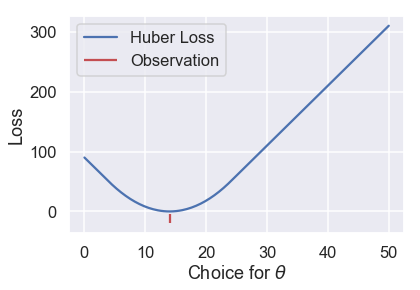
\includegraphics[width=0.85\textwidth]{huber}
\caption*{}
\end{figure}
\vspace{-10mm}
\begin{align*}
L_\delta(\theta, \textbf{y}) = \frac{1}{n} \sum_{i=1}^n 
\begin{cases}
    \frac{1}{2}(y_i - \theta)^2 &  | y_i - \theta | \le \delta \\
    \delta ( |y_i - \theta| - \frac{1}{2}\delta ) & \text{otherwise}
\end{cases}
\end{align*}
\column{0.4\textwidth}
What does this buy us?
\pause
\begin{itemize}
\item Differentiable
\item Absolute value at extremes -- not dominated by outlier.
\end{itemize}

\vspace{5mm}
\pause
What does this cost us?
\pause
\begin{itemize}
\item There is no ``closed form'' solution (e.g. no equivalent to normal equations).
\end{itemize}
\end{columns}
\end{frame}

\begin{frame}{Estimation takeaway \# 1: }

Analytical solutions for parameters (e.g. by setting partial derivatives equal to zero) not always available for some of the types of loss functions we'd like to use.
\end{frame}

\begin{frame}{Estimation takeaway \# 2: }

A separate issue: In situations where the normal equations (or something like them) can be used to solve for parameters:

\begin{align*}
\Theta &=  
(X^TX)^{-1}X^TY
\end{align*}

It can be very difficult computationally to invert a large $X^TX$ (On my computer, Python can't deal with with 50,000 by 50,000).  
\end{frame}



\begin{frame}{Gradient descent -- sketch}

\pause
\begin{figure}
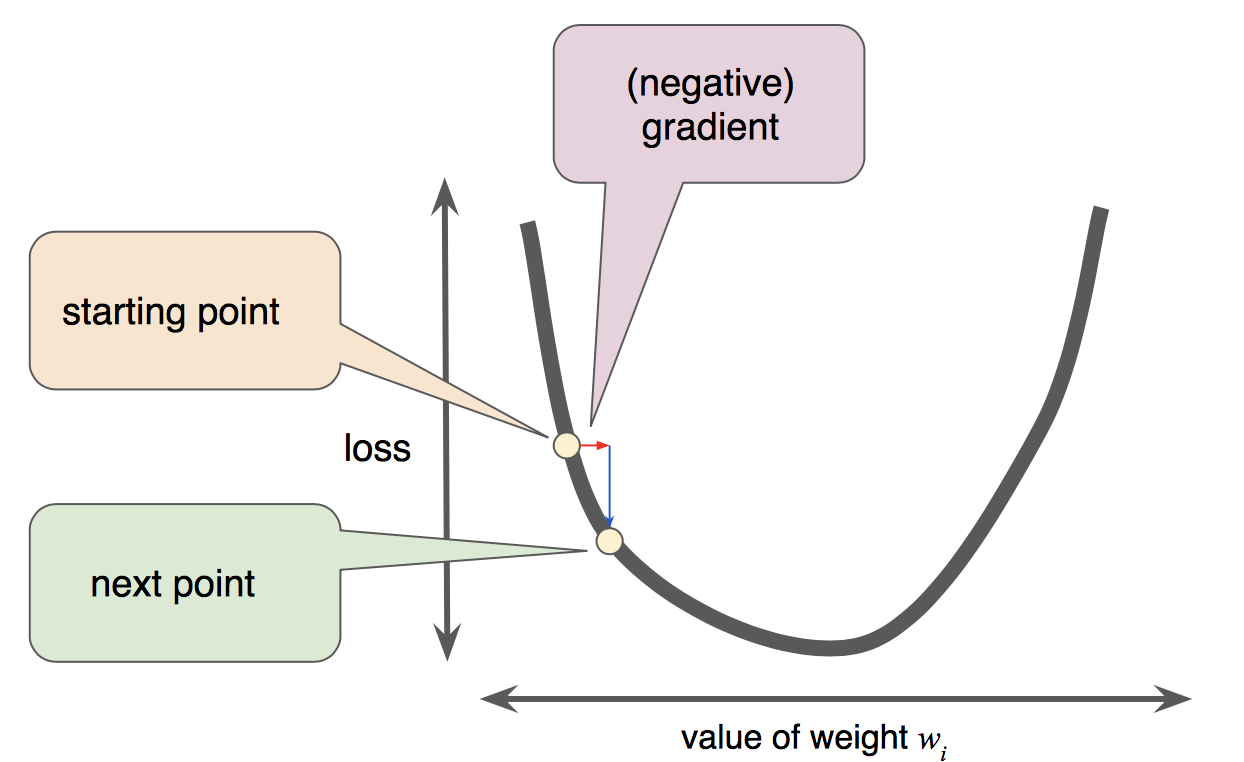
\includegraphics[height=0.7\textheight]{grad_desc_google_4}
\caption*{\url{https://developers.google.com/machine-learning/crash-course/reducing-loss/gradient-descent}}
\end{figure}

\end{frame}



\begin{frame}{Gradient descent -- math}

What's the gradient?  For our purposes, it is the slope of the loss function at a given point \textit{with respect to a particular parameter.}

\vspace{10mm}

The gradient is $\nabla_\theta L(\theta, \textbf{y}) = \uncover<2->{\frac{\partial}{\partial \theta} L(\theta, \textbf{y}).}$

\vspace{10mm}

\textbf{Gradient descent process}:
\begin{enumerate}
\item Choose a value for the ``learning rate'', $\alpha$
\item Choose a starting value of  $\theta$ (0 is a common choice).
\item Compute  $\theta - \alpha \cdot \frac{\partial}{\partial \theta} L(\theta, \textbf{y})$ and store this as the new value of $\theta$.  
\item Repeat until $\theta$ doesn't change (much) between iterations.
\end{enumerate}

\vspace{5mm}

\end{frame}

\begin{frame}{Gradient descent for quadratic loss}

\begin{columns}
\column{0.5\textwidth}
Let's derive the gradient:
\pause
\uncover<2->{
\begin{align*}
L &= \sum_{i=1}^n (y_i-\theta)^2\\
\frac{\partial L}{\partial \theta} & =  -2\sum_{i=1}^n (y_i-\theta)
\end{align*}
}
\column{0.5\textwidth}
...and then write a few iterations: 
\uncover<3->{\begin{align*}
\Rightarrow & \theta_1=0\\
					&\theta_2 = \theta_1 - \alpha(-2\sum_{i=1}^n (y_i-\theta_1))\\
					&\vdots\\
					&\theta_{t+1} = \theta_t - \alpha(-2\sum_{i=1}^n (y_i-\theta_t))
\end{align*}
Stop when $|\theta_{t+1} - \theta_t| < \text{tol}$, where ``tol'' is a small tolerance parameter.}
\end{columns}
\end{frame}

\begin{frame}{Gradient descent, in code}

%
%In other words:
%
%\vspace{5mm}
%
%$\theta^{(t+1)} = \theta^{(t)} - \alpha \cdot \nabla_\theta L(\theta^{(t)}, \textbf{y})$

\begin{figure}
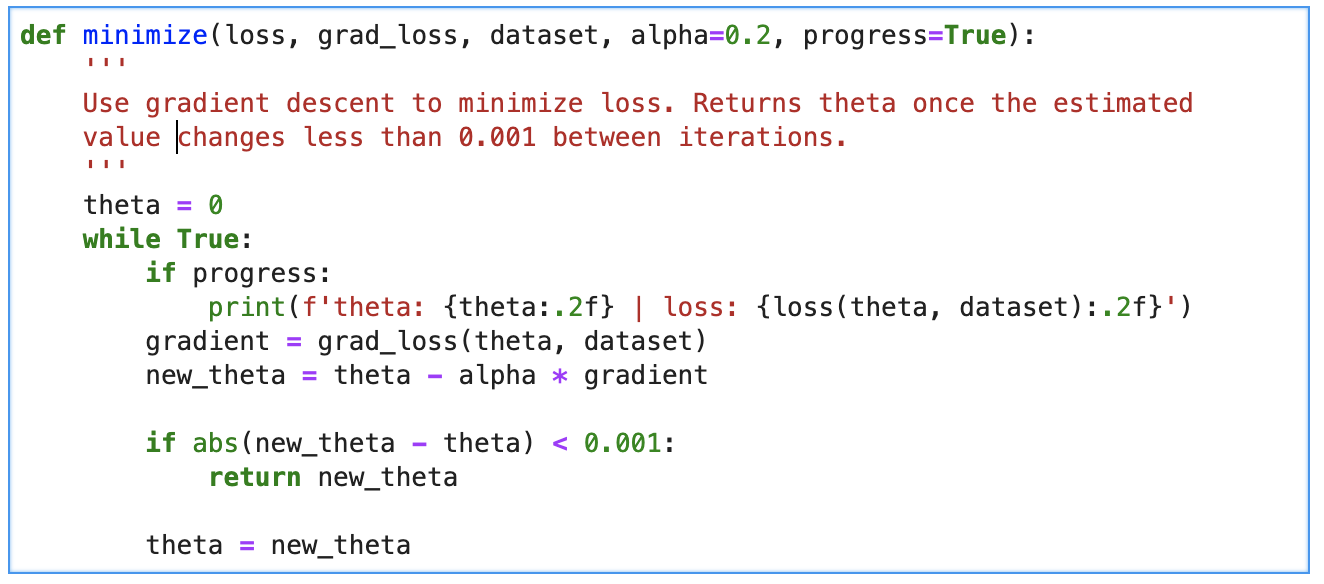
\includegraphics[width=1.\textwidth]{grad_desc}
%\caption*{\url{https://www.textbook.ds100.org/ch/11/gradient_descent_define.html}}
\end{figure}

\end{frame}

\begin{frame}{Gradient descent -- what does the learning rate do?}

Get in small groups and play with this Google tool: \href{https://goo.gl/JNPhUv}{https://goo.gl/JNPhUv}.

\vspace{5mm}

Set $\alpha$ to a higher value than the default -- it'll take forever at $\alpha = 0.01$.  
\vspace{5mm}

Questions to answer together:  How does the rate change on each iteration...
\begin{enumerate}
\item ...when the learning rate is really small?
\item ...when the learning rate is really big?
\end{enumerate}

\end{frame}

\begin{frame}{Types of gradient descent trajectories}

\begin{columns}
\column{0.4\textwidth}
There are four qualitatively different behaviors:
\begin{enumerate}
\item Monotonically decreasing loss
\item One step to optimal parameter
\item Loss declines in periodic oscillations
\item Loss grows out of control
\end{enumerate}

\column{0.6\textwidth}

\end{columns}

\end{frame}

\begin{frame}{What do you think the point of a ``dynamic learning rate" might be?}

\pause

Basic idea: Start with a big learning rate, then make it smaller and smaller as you approach the optimal value

\pause

\vspace{10mm}

Advantages: 
\begin{itemize}
\item cover a lot of ground when you're far from the optimal value
\item refined steps when you get close, so you don't miss the optimal value.
\end{itemize}

\end{frame}


\begin{frame}{Gradient descent -- absolute deviation loss, ctd.}

\begin{columns}
\column{0.5\textwidth}
  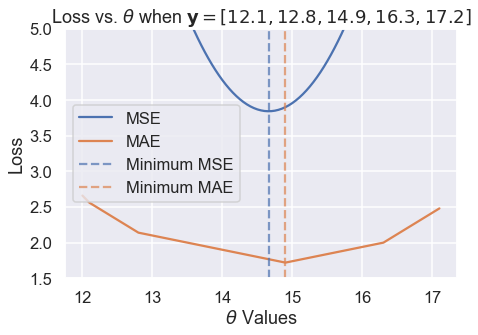
\includegraphics[width=\textwidth]{mae_vs_mse}

\column{0.5\textwidth}

What's the problem with doing gradient descent here?

\vspace{5mm}

\pause

The derivative does not go to zero at the optimal value.  

\vspace{5mm}

So once the solution is close, it won't converge, unless...\pause we use a dynamic learning rate.
\end{columns}

\end{frame}

\begin{frame}{Novotny Questions}
\begin{enumerate}
  \item Describe the basic model selection process and how it differs from AIC (which we learned briefly in class on Thursday).  This question can be answered if you read Section 2.2 and 2.3 carefully and do a little background research to understand unfamiliar terms. 
  \item The authors compare R2 values for the test data versus R2 for the training data.  What do they obeserve?  What does this imply about their data and model?  Read Section 3.3 to answer this question.  
  \item  Also in section 3.3 the authors state "We also investigated the extent to which monitor locations span the (independent) variable space, an important issue for any LUR".  What does this mean?  Why is spanning the variable space important?
  \item The authors discuss several limitations in the Discussion section.  Review these.  How important are their limitations?  Are there others you think are worth considering?
\end{enumerate}
\end{frame}

\begin{frame}{Novotny answers}
\begin{enumerate}
  \item Model selection:
  \begin{itemize}
    \item build model by adding variables sequentially
    \item variable most correlated with \textit{residuals} from prior model added to next candidate
    \item variables stay in the model if $p<0.05$ and VIF$<5$
    \item stop when the next added independent variable would not be statistically significant or would fail the VIF multicollinearity check
  \end{itemize}
  Note, in my opinion this misses the mark for what we \textit{should} be doing.  Any guesses why?
  \pause
  \begin{itemize}
    \item They should only care about test error.  
  \end{itemize}
  
\end{enumerate}
\end{frame}



\begin{frame}{Novotny answers}


2. They find R2 for test error is comparable to training --> they are not overfitting the model.  But could they do better?

3. ``spanning the variable space'' is important for validity of the prediction model.  Trying to predict variables outside of the range you used to build your model raises questions about external validity.

4. 
\begin{itemize}
  \item ``we do not investigate sources such as industry, airports, or harbors''
  \item ``our model is derived from road length rather than traffic volumes''
  \item ``our model performance evaluations employ the data used to derive the model''
  \item ``our model only predicts outdoor concentrations''
\end{itemize}


\end{frame}
\end{document}


